You literally just try to build a hyperplane to minimize the number of misclassifications, but this is not really differentiable and is hard. It's just a stepwise function. Therefore, you use a \textbf{surrogate loss function} to approximate the 0-1 loss function. The logistic uses some function, and the SVM uses the smallest convex function to approximate the 0-1 loss function. Here are some examples: 

\begin{figure}[H]
  \centering
  \begin{subfigure}[b]{0.48\textwidth}
    \centering
    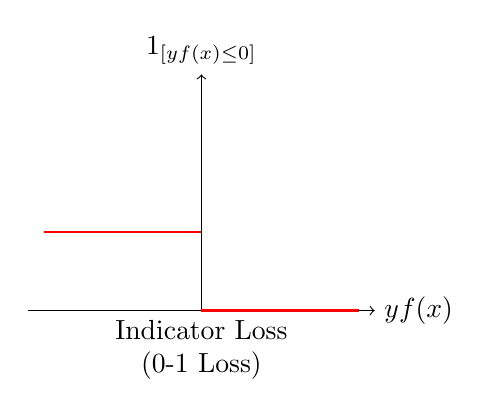
\begin{tikzpicture}
      \draw[->] (-2.2,0) -- (2.2,0) node[right] {$yf(x)$};
      \draw[->] (0,0) -- (0,3) node[above] {$1_{[yf(x)\leq0]}$};
      \draw[red, thick] (-2,1) -- (0,1);
      \draw[red, thick] (0,0) -- (2,0);
      \node[align=center] at (0,-0.5) {Indicator Loss\\(0-1 Loss)};
    \end{tikzpicture}
    \caption{Indicator/0-1 Loss can't be easily optimized.}
    \label{fig:indicator}
  \end{subfigure}
  \begin{subfigure}[b]{0.48\textwidth}
    \centering
    \begin{tikzpicture}
      \draw[->] (-2.2,0) -- (2.2,0) node[right] {$yf(x)$};
      \draw[->] (0,0) -- (0,3) node[above] {$e^{-yf(x)}$};
      \draw[green!50!black, thick, domain=-2:2, samples=100] 
        plot (\x, {0.5*exp(-0.7*\x)});
    \end{tikzpicture}
    \caption{Exponential Loss for Adaboost.}
    \label{fig:exponential}
  \end{subfigure}
  
  \begin{subfigure}[b]{0.48\textwidth}
    \centering
    \begin{tikzpicture}
      \draw[->] (-2.2,0) -- (2.2,0) node[right] {$yf(x)$};
      \draw[->] (0,0) -- (0,3) node[above] {$\log(1+e^{-yf(x)})$};
      \draw[blue, thick, domain=-2:2, samples=100] 
        plot (\x, {ln(1 + exp(-\x))});
    \end{tikzpicture}
    \caption{Log Loss for logistic regression. }
    \label{fig:logistic}
  \end{subfigure}
  \begin{subfigure}[b]{0.48\textwidth}
    \centering
    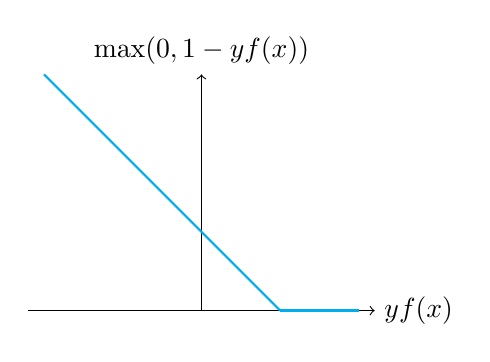
\begin{tikzpicture}
      \draw[->] (-2.2,0) -- (2.2,0) node[right] {$yf(x)$};
      \draw[->] (0,0) -- (0,3) node[above] {$\max(0,1-yf(x))$};
      \draw[cyan, thick] (-2,3) -- (1,0);
      \draw[cyan, thick] (1,0) -- (2,0);
    \end{tikzpicture}
    \caption{Hinge Loss for support vector machines.}
    \label{fig:hinge}
  \end{subfigure}
  \caption{Common loss functions used in classification}
  \label{fig:loss_functions}
\end{figure}

